\documentclass[english]{article}

\usepackage[latin9]{inputenc}
\usepackage[letterpaper]{geometry}
\geometry{verbose,tmargin=.8in,bmargin=1in,lmargin=1in,rmargin=1in}
\usepackage{amsmath}
\usepackage{amssymb}
\usepackage{graphicx}
%\usepackage{pdftk}
\usepackage{multicol}
\usepackage{float}
\usepackage{array}
\usepackage{tikz}
\usepackage{multirow}

\title{1D electromagnets for control of 2 permanent magnetics analysis}
\author{Denise Wong}

\begin{document}
\maketitle
\begin{center}
\includegraphics[width=5in]{1Dprobsetup.JPG}
\end{center}

\section{System setup}
$\mu_0$ : permeability constant $4\pi \times 10^{-7} Tm/A$\\
$\vec{\mu_j}$ : magnetic dipole moment for magnet j, $Am^2$\\
$I_i$ : current through coil i, A\\
$R_i$ : radius of coil i, m\\
$C_{perm} = \frac{\mu_0 I_p R_p^2}{2}$ : constant representing permanent magnet strength

\subsection{Electromagnet}
The magnetic field on-axis of the coil is given by:
$${B}_{loop} = \frac{\mu_0 I R^2}{2\left(z^2 + R^2\right)^{3/2}}$$
${z}$ : distance from the center of the fixed electromagnet to the center of the free permanent magnet.  

\subsection{Permanent Magnet}
\subsection*{Permanent Magnet modeled using classical mechanics}
Let force between 2 magnets be expressed as:
$$\vec{F} = \frac{\mu_0 m_1 m_2}{4 \pi r^2}\hat{r}$$
where $m_1,m_2$ are the magnitude of the magnetic poles of permanent magnet 1 and 2 measured in Ampere-meters (Am).  Written in the above coordinate frame for the 1D problem, the force in the x-direction acting on magnet 1:
$$F_{x,1} = \frac{\mu_0 m_1 m_2}{4 \pi \left(x_2-x_1\right)^2}$$


%\subsection*{Permanent Magnet as an electromagnet}
%Model the magnetism of the permanent magnet as a magnet field produced from currents within the magnet(e.g. permanent internal currents.)
%$${B}_{perm} = \frac{\mu_0 I R_p^2}{2\left(z^2 + R_p^2\right)^{3/2}} = C_{perm} \frac{1}{\left(z^2 + R_p^2\right)^{3/2}}$$
%
%$C_{perm} = \frac{\mu_0 I_p R_p^2}{2}$ is a constant for a permanent magnet. 
%%\section*{Force on each magnet}

\section{Force exerted on each magnet}
Relating the magnetic field, $\vec{B}$ to the force, F:
$$F = \vec{\mu}\cdot\nabla\vec{B}$$
$$\vec{B} = \frac{\mu_0 I R^2}{2 \left(x^2 + R^2\right)^{3/2}}, \nabla\vec{B} = \frac{dB}{dx} =  \frac{3x\mu_0IR^2}{2\left(x^2 + R^2\right)^{5/2}}$$
For a 1D system as shown above, this simplifies to:
$$F_x = \mu\frac{d\vec{B}}{dx}$$
The force exerted on magnet 1 is given by:
$$F_{x,1} = \mu_1\left(-\frac{3 x_1 \mu_0 I_1 R_{1}^{2}}{2\left(x_1^2 + R_1^2 \right)^{\frac{5}{2}}} - \frac{3 \left( x_1 - L \right) \mu_0 I_2 R_{2}^{2}}{2\left(\left(x_1 - L \right)^2 + R_2^2 \right)^{\frac{5}{2}}} \right) + \frac{\mu_0 m_1 m_2}{4 \pi \left(x_2-x_1\right)^2}$$
The force exerted on magnet 2 is given by:
$$F_{x,2} = \mu_2\left(-\frac{3 x_2 \mu_0 I_1 R_{1}^{2}}{2\left(x_2^2 + R_1^2 \right)^{\frac{5}{2}}} - \frac{3 \left( x_2 - L \right) \mu_0 I_2 R_{2}^{2}}{2\left(\left(x_2 - L \right)^2 + R_2^2 \right)^{\frac{5}{2}}} \right) - \frac{\mu_0 m_1 m_2}{4 \pi \left(x_1-x_2\right)^2}$$
Writing this in matrix form:
\begin{equation}
\begin{bmatrix}
	F_{x,1}\\[0.3em]
	F_{x,2}	
\end{bmatrix}
=
\begin{bmatrix}
			-\mu_1\frac{3 x_1 \mu_0 R_{1}^{2}}{2\left(x_1^2 + R_1^2 \right)^{\frac{5}{2}}}  & -\mu_1\frac{3 \left( x_1 - L \right) \mu_0 R_{2}^{2}}{2\left(\left(x_1 - L \right)^2 + R_2^2 \right)^{\frac{5}{2}}} & 	\frac{\mu_0 m_1 m_2}{4\pi \left(x_2-x_1\right)^2}\\
			-\mu_2\frac{3 x_2 \mu_0 R_{1}^{2}}{2\left(x_2^2 + R_1^2 \right)^{\frac{5}{2}}} & -\mu_2\frac{3 \left( x_2 - L \right) \mu_0 R_{2}^{2}}{2\left(\left(x_2 - L \right)^2 + R_2^2 \right)^{\frac{5}{2}}} & 	-\frac{\mu_0 m_1 m_2}{4\pi \left(x_2-x_1\right)^2}\\
\end{bmatrix}
\begin{bmatrix}
	I_1\\ I_2 \\ 1
\end{bmatrix}
\label{eq:ForceMatrix_general}
\end{equation}

Setting the above force equations so that force is 0 to find the equilibrium point and writing these 2 equations in matrix form to solve for the input current given a starting configuration:

\begin{center}
$\begin{bmatrix}
	-\frac{\mu_0 m_1 m_2}{4\pi \left(x_2-x_1\right)^2} \\[0.3em]
	\frac{\mu_0m_1m_2}{4\pi \left(x_2-x_1\right)^2}	
\end{bmatrix}
$=$
\begin{bmatrix}
			-\mu_1\frac{3 x_1 \mu_0 R_{1}^{2}}{2\left(x_1^2 + R_1^2 \right)^{\frac{5}{2}}}  & -\mu_1\frac{3 \left( x_1 - L \right) \mu_0 R_{2}^{2}}{2\left(\left(x_1 - L \right)^2 + R_2^2 \right)^{\frac{5}{2}}}\\
			-\mu_2\frac{3 x_2 \mu_0 R_{1}^{2}}{2\left(x_2^2 + R_1^2 \right)^{\frac{5}{2}}} & -\mu_2\frac{3 \left( x_2 - L \right) \mu_0 R_{2}^{2}}{2\left(\left(x_2 - L \right)^2 + R_2^2 \right)^{\frac{5}{2}}}\\
\end{bmatrix}
\begin{bmatrix}
	I_1\\ I_2
\end{bmatrix}
$
\end{center}

By inspecting the determinant of the 2x2 matrix, it can be shown that a solution for the 2 currents through the coil exists as long as $x_1 \neq x_2$, a configuration that is not physically possible.

\section{Potential Function}
The potential function can be used to explore the stability of a system.  It is related to the force on a system by:
$$ F = -\frac{dU}{dx}$$
Given that for magnets, $\vec{F_j} = \vec{\mu_j} \bullet \frac{d\vec{B}}{dx}$, the potential function, U, is a function of the magnetic field, B.  Assuming that $\vec{\mu}_j$ is a constant, the potential function in the x direction for the j-th permanent magnet: \\
$$ U_{x,j} = -\int_{x_i}^{x} F_x dx + U(x_i) = - \mu_{x,j}B_x$$

%%% ---------------------- %%%%
%\subsection*{Permanent magnet modeled as electromagnet}
%The magnetic field on the j-th permanent magnet:
%$$B_{x,j} = \frac{\mu_0 I_1 R_{1}^{2}}{2 \left(x_j^2 + R_1^2 \right)^{\frac{3}{2}}} + \frac{\mu_0 I_2 R_{2}^{2}}{2 \left(\left(x_j - L \right)^2 + R_2^2 \right)^{\frac{3}{2}}} + C_{perm}\frac{1}{\left(\left(x_j-x_k\right)^2  +R_p^2\right)^{\frac{3}{2}}}$$
%
%Potential function in the x-direction along the axis of the electromagnetic coils for 1st magnet:
%$$ U = \mu_1\left(\frac{\mu_0 I_1 R_{1}^{2}}{2 \left(x_1^2 + R_1^2 \right)^{\frac{3}{2}}} + \frac{\mu_0 I_2 R_{2}^{2}}{2 \left(\left(x_1 - L \right)^2 + R_2^2 \right)^{\frac{3}{2}}} + C_{perm}\frac{1}{\left(\left(x_1-x_2\right)^2  +R_p^2\right)^{\frac{3}{2}}}\right)$$
%%%% ---------------------- %%%%


\subsection{Permanent magnet modeled using classical mechanics}
To compute the potential function component from this interaction:
$$U_{perm} = -\int_{x_i}^{x}F dx + U\left(x_i\right) = -\int_{x_i}^{x_1}\frac{\mu_0 m_1 m_2}{4 \pi \left(x_2-x_1\right)^2} dx_1 + U\left( x_i \right) = -\left[-\frac{\mu_0 m_1 m_2}{4\pi \left(x_1 - x_2\right)} \right]_{x_i}^{x_1} + U\left(x_i\right)$$
Letting $-\frac{\mu_0 m_1 m_2}{4\pi \left(x_i - x_2\right)} + U\left(x_i\right) = 0$.  

The expression for the potential function for magnet 1 in the above system is therefore:
$$U_1 = \mu_1\left(\frac{\mu_0 I_1 R_{1}^{2}}{2 \left(x_1^2 + R_1^2 \right)^{\frac{3}{2}}} + \frac{\mu_0 I_2 R_{2}^{2}}{2 \left(\left(x_1 - L \right)^2 + R_2^2 \right)^{\frac{3}{2}}} \right) + \frac{\mu_0 m_1 m_2}{4\pi \left(x_2 - x_1\right)}$$


The expression for the potential function for magnet 2 in the above system is therefore:
$$U_2 = \mu_1\left(\frac{\mu_0 I_1 R_{1}^{2}}{2 \left(x_2^2 + R_1^2 \right)^{\frac{3}{2}}} + \frac{\mu_0 I_2 R_{2}^{2}}{2 \left(\left(x_2 - L \right)^2 + R_2^2 \right)^{\frac{3}{2}}} \right) + \frac{\mu_0 m_1 m_2}{4\pi \left(x_1 - x_2\right)}$$

\subsection{Stability analysis}
By looking at one specific case where, we can see that the equilibrium is not stable.  This agrees with intuition.

For a coil separation of L = 0.10 m with coils of radius R = 0.01 
To hold 2 magnets at x = 0.03 and 0.05 m
Current needed: I1 =  0.0880 A, I2 =  0.4331 A
\begin{figure}[H]
	\centering
	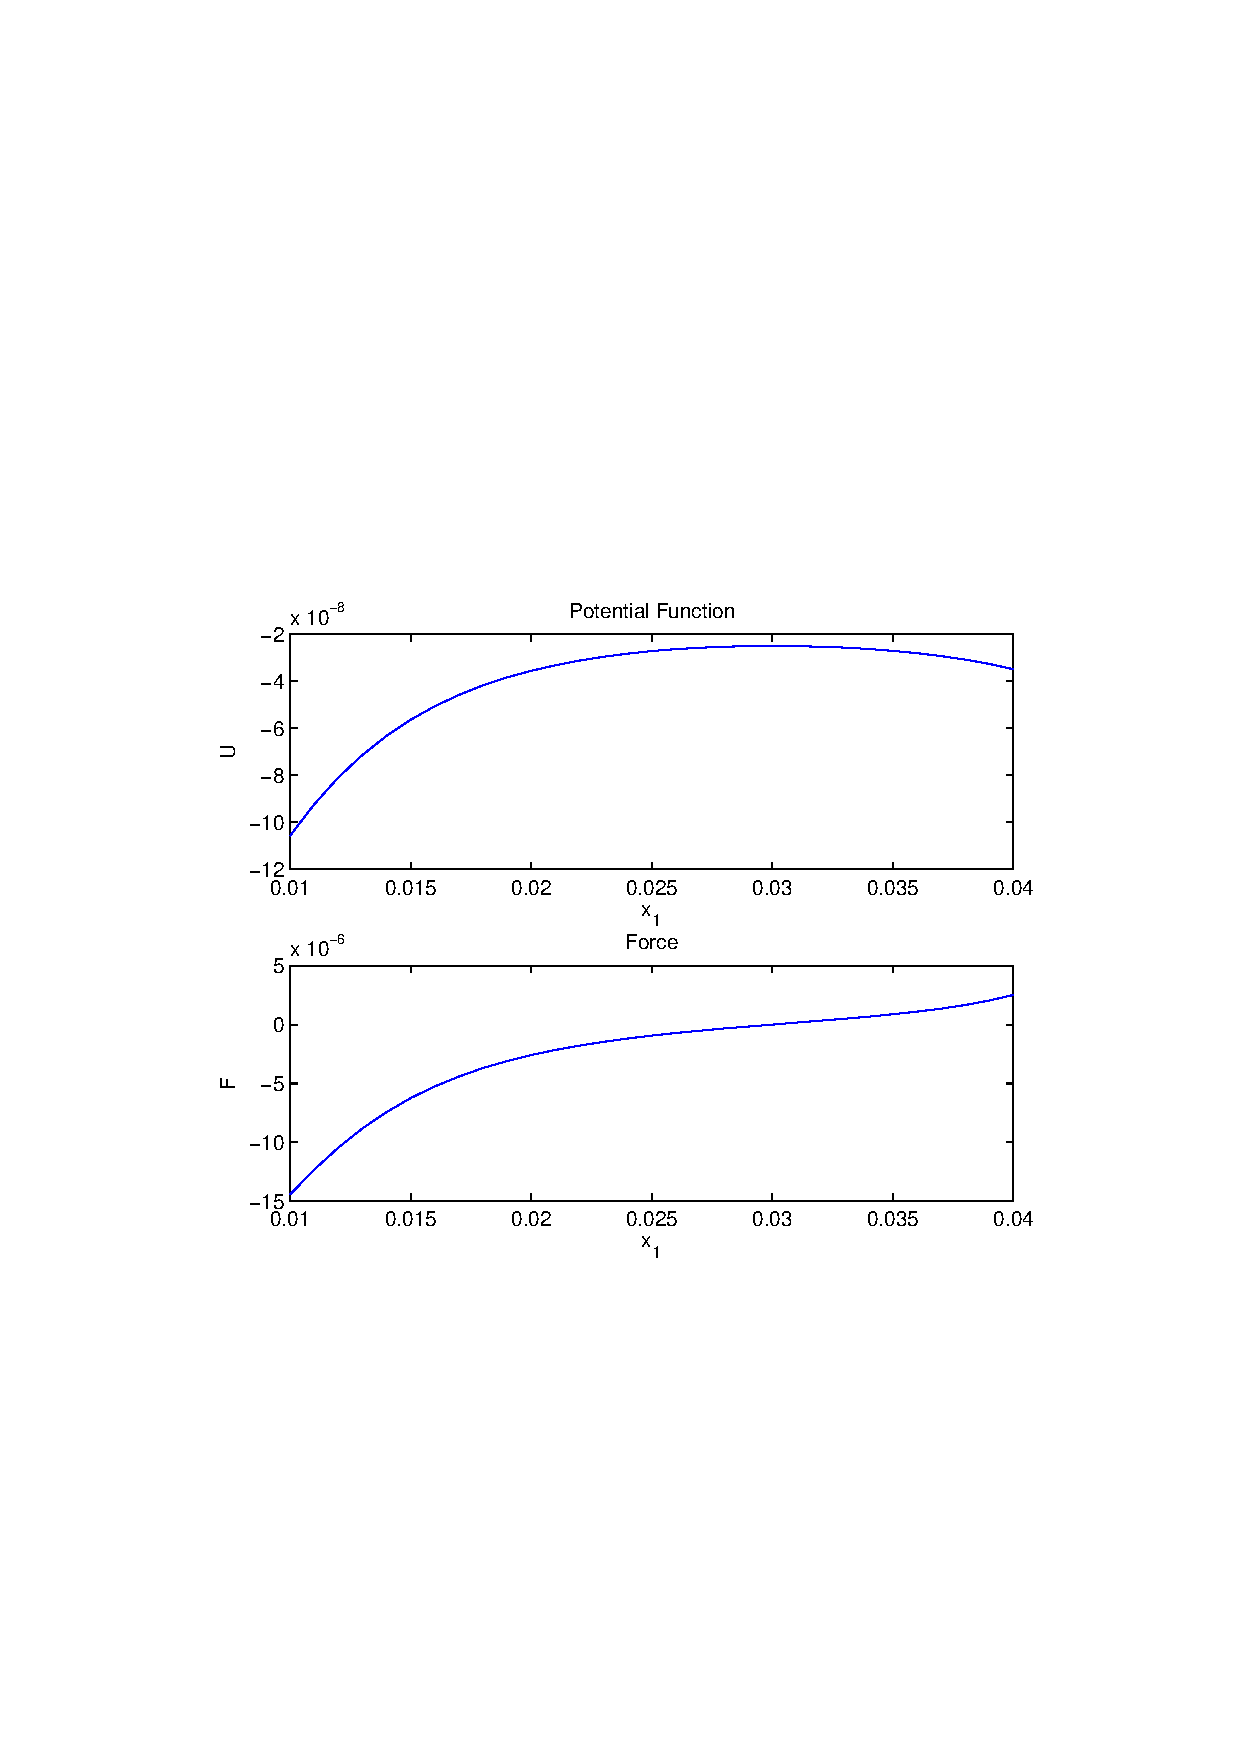
\includegraphics[width = 5in]{figures/UF_unstable.pdf}
\end{figure}


The Hessian matrix is computed to determine the stability of the equilibrium point, where $\frac{dU}{dx_1}=0$:

$$H = \begin{bmatrix}
	\frac{\partial ^2 U}{\partial x_1^2} & \frac{\partial ^2 U}{\partial x_1 \partial x_2}\\
	\frac{\partial ^2 U}{\partial x_2 \partial x_1} & \frac{\partial ^2 U}{\partial x_2^2}
\end{bmatrix}
$$

For magnet 1:
$$H_1 = \begin{bmatrix}
	\frac{\partial ^2 U_1}{\partial x_1^2} & \frac{\partial ^2 U_1}{\partial x_1 \partial x_2}\\
	\frac{\partial ^2 U_1}{\partial x_2 \partial x_1} & \frac{\partial ^2 U_1}{\partial x_2^2}
\end{bmatrix}
\\=
\begin{bmatrix}
	\left(\frac{-3}{\left(\left(x_1 - L\right)^2 + R_2^2\right)^{\frac{5}{2}}} + \frac{15\left(x_1-L\right)^2}{\left(\left(x_1 - L\right)^2 + R_2^2\right)^{\frac{7}{2}}} + \frac{15x_1^2}{\left(R_1^2 + x_1^2 \right)^{\frac{7}{2}}} - \frac{3}{\left(R_1^2 + x_1^2 \right)^{\frac{5}{2}}} + \frac{2}{\left(x_2-x_1\right)^3}\right)
	& 
	-\frac{2}{\left(x_2-x_1\right)^3}\\
	-\frac{2}{\left(x_2-x_1\right)^3}
	&
	\frac{2}{\left(x_2-x_1\right)^3}
\end{bmatrix}
$$

For magnet 2:
$$H_2 = \begin{bmatrix}
	\frac{\partial ^2 U_2}{\partial x_1^2} & \frac{\partial ^2 U_2}{\partial x_1 \partial x_2}\\
	\frac{\partial ^2 U_2}{\partial x_2 \partial x_1} & \frac{\partial ^2 U_2}{\partial x_2^2}
\end{bmatrix}
\\=
\begin{bmatrix}
	\frac{2}{\left(x_1-x_2\right)^3}	
	& 
	-\frac{2}{\left(x_1-x_2\right)^3}\\
	-\frac{2}{\left(x_1-x_2\right)^3}
	&
	\left(\frac{-3}{\left(\left(x_2 - L\right)^2 + R_2^2\right)^{\frac{5}{2}}} + \frac{15\left(x_2-L\right)^2}{\left(\left(x_2 - L\right)^2 + R_2^2\right)^{\frac{7}{2}}} + \frac{15x_2^2}{\left(R_1^2 + x_2^2 \right)^{\frac{7}{2}}} - \frac{3}{\left(R_1^2 + x_2^2 \right)^{\frac{5}{2}}} + \frac{2}{\left(x_1-x_2\right)^3}\right)
\end{bmatrix}
$$

Solving for the eigenvalues:
...
will show that equilibrium points are unstable.

\section{Non-dimensionalizing Force Expression}
Taking the most general form of the force expression \ref{eq:ForceMatrix_general}, we can make some assumptions to simplify the expression; then we will non-dimensionalize the system of equations to study system characteristics.  First, the system geometry is generalized such that:

\begin{itemize}\itemsep1pt \parskip0pt \parsep1pt
\item{Size of all the coils are the same $R_1 = R_2 = R$}
\item{Magnetic dipole moment for permanent magnets are the same $\mu_1 = \mu_2 = \mu$}
\item{Magnetic pole magnitude for permanent magnets are the same $m_1 = m_2 = m$}
\end{itemize}


\begin{equation}
\begin{bmatrix}
	F_{x,1}\\[0.3em]
	F_{x,2}	
\end{bmatrix}
=
\begin{bmatrix}
			-\mu\frac{3 x_1 \mu_0 R^{2}}{2\left(x_1^2 + R^2 \right)^{\frac{5}{2}}}  & -\mu\frac{3 \left( x_1 - L \right) \mu_0 R^{2}}{2\left(\left(x_1 - L \right)^2 + R^2 \right)^{\frac{5}{2}}} & 	\frac{\mu_0 m^2}{4\pi \left(x_2-x_1\right)^2}\\
			-\mu\frac{3 x_2 \mu_0 R^{2}}{2\left(x_2^2 + R^2 \right)^{\frac{5}{2}}} & -\mu_2\frac{3 \left( x_2 - L \right) \mu_0 R^{2}}{2\left(\left(x_2 - L \right)^2 + R^2 \right)^{\frac{5}{2}}} & 	-\frac{\mu_0 m^2}{4\pi \left(x_2-x_1\right)^2}\\
\end{bmatrix}
\begin{bmatrix}
	I_1\\ I_2 \\ 1
\end{bmatrix}
\label{eq:ForceMatrix_assumptions}
\end{equation}

Now to nondimensionalize the equations, we define the variables with units:\\
\begin{center}
$\begin{array}{lll}
\tilde{x_i} &= \frac{\tilde{x_j}}{R} &\left[=\right] dimensionless\\
\alpha &= \frac{L}{R} &\left[=\right] dimensionless \\
\tilde{I_j} &= \frac{\mu_0 \mu I_j}{R^2} &\left[ = \right] N\\
\tilde{F_i} &= F_i &\left[ = \right] N
\end{array}$
\end{center}


\begin{equation}
\begin{bmatrix}
	\tilde{F}_{x,1}\\[0.3em]
	\tilde{F}_{x,2}	
\end{bmatrix}
=
\begin{bmatrix}
			-\frac{3\mu}{2} \frac{\tilde{x}_1}{\left(\tilde{x}_1^2 + 1 \right)^{\frac{5}{2}}}  & -\frac{3\mu}{2}\frac{\frac{1}{\alpha}\left(\alpha\tilde{x_1} - 1 \right)}{\left(\frac{1}{\alpha^2}\left(\alpha \tilde{x_1} - 1 \right)^2 + 1 \right)^{\frac{5}{2}}} & 	\left(\tilde{x_2}-\tilde{x_1}\right)^{-2}\\
			-\frac{3\mu}{2} \frac{\tilde{x}_2}{\left(\tilde{x}_2^2 + 1 \right)^{\frac{5}{2}}}  & -\frac{3\mu}{2}\frac{\frac{1}{\alpha}\left(\alpha\tilde{x_2} - 1 \right)}{\left(\frac{1}{\alpha^2}\left(\alpha \tilde{x_2} - 1 \right)^2 + 1 \right)^{\frac{5}{2}}} & 	-\left(\tilde{x_2}-\tilde{x_1}\right)^{-2}\\
\end{bmatrix}
\begin{bmatrix}
	\tilde{I}_1\\ \tilde{I}_2 \\ \frac{\mu_0 m^2}{4 \pi R^2}
\end{bmatrix}
\label{eq:ForceMatrix_nondim}
\end{equation}

From equation \ref{eq:ForceMatrix_nondim} we want to show that the 2x3 matrix has a rank of 2 for 2DOF control.

We can do this by computing the determinant of the 2x2 matrix on the left which include the coefficients that multiply $\tilde{I_1}$ and $\tilde{I_2}$.  

$\begin{array}{ll}
\det \begin{vmatrix}
			-\frac{3\mu}{2} \frac{\tilde{x}_1}{\left(\tilde{x}_1^2 + 1 \right)^{\frac{5}{2}}}  & 
			-\frac{3\mu}{2}\frac{\frac{1}{\alpha}\left(\alpha\tilde{x_1} - 1 \right)}{\left(\frac{1}{\alpha^2}\left(\alpha \tilde{x_1} - 1 \right)^2 + 1 \right)^{\frac{5}{2}}} 
			\\
			-\frac{3\mu}{2} \frac{\tilde{x}_2}{\left(\tilde{x}_2^2 + 1 \right)^{\frac{5}{2}}} & 
			-\frac{3\mu}{2}\frac{\frac{1}{\alpha}\left(\alpha\tilde{x_2} - 1 \right)}{\left(\frac{1}{\alpha^2}\left(\alpha \tilde{x_2} - 1 \right)^2 + 1 \right)^{\frac{5}{2}}}
\end{vmatrix} &= 
\frac{9\mu^2}{4} \left(\frac{\tilde{x}_1}{\left(\tilde{x}_1^2 + 1 \right)^{\frac{5}{2}}}\frac{\frac{1}{\alpha}\left(\alpha\tilde{x_2} - 1 \right)}{\left(\frac{1}{\alpha^2}\left(\alpha \tilde{x_2} - 1 \right)^2 + 1 \right)^{\frac{5}{2}}} - \frac{\frac{1}{\alpha}\left(\alpha\tilde{x_1} - 1 \right)}{\left(\frac{1}{\alpha^2}\left(\alpha \tilde{x_1} - 1 \right)^2 + 1 \right)^{\frac{5}{2}}}\frac{\tilde{x}_2}{\left(\tilde{x}_2^2 + 1 \right)^{\frac{5}{2}}} \right)\\
&= \frac{9\mu^2}{4}\left( \frac{\tilde{x}_1 \tilde{x}_2 - \frac{\tilde{x}_1}{\alpha}}{\left[\left(\tilde{x}_1^2 + 1 \right) \left( \frac{1}{\alpha^2}\left(\alpha \tilde{x}_2 -1\right)^2 + 1\right) \right]^{\frac{5}{2}}} - \frac{\tilde{x}_1 \tilde{x}_2 - \frac{\tilde{x}_2}{\alpha}}{\left[\left(\tilde{x}_2^2 + 1 \right) \left( \frac{1}{\alpha^2}\left(\alpha \tilde{x}_1 -1\right)^2 + 1\right) \right]^{\frac{5}{2}}}\right)\\
&=
\frac{9 \tilde{x}_2 \alpha ^5 \sqrt{\frac{1-2 \tilde{x}_1 \alpha +\alpha ^2+\tilde{x}_1^2 \alpha ^2}{\alpha ^2}}}{4
\left(1+\tilde{x}_2^2\right)^{5/2} \left(1-2 \tilde{x}_1 \alpha +\alpha ^2+\tilde{x}_1^2 \alpha ^2\right)^3}-\frac{9 \tilde{x}_1 \tilde{x}_2 \alpha ^6 \sqrt{\frac{1-2
\tilde{x}_1 \alpha +\alpha ^2+\tilde{x}_1^2 \alpha ^2}{\alpha ^2}}}{4 \left(1+\tilde{x}_2^2\right)^{5/2} \left(1-2 \tilde{x}_1 \alpha +\alpha ^2+\tilde{x}_1^2
\alpha ^2\right)^3}\\
&-
\frac{9 \tilde{x}_1 \alpha ^5 \sqrt{\frac{1-2 \tilde{x}_2 \alpha +\alpha ^2+\tilde{x}_2^2 \alpha ^2}{\alpha ^2}}}{4 \left(1+\tilde{x}_1^2\right)^{5/2}
\left(1-2 \tilde{x}_2 \alpha +\alpha ^2+\tilde{x}_2^2 \alpha ^2\right)^3}+\frac{9 \tilde{x}_1 \tilde{x}_2 \alpha ^6 \sqrt{\frac{1-2 \tilde{x}_2 \alpha +\alpha
^2+\tilde{x}_2^2 \alpha ^2}{\alpha ^2}}}{4 \left(1+\tilde{x}_1^2\right)^{5/2} \left(1-2 \tilde{x}_2 \alpha +\alpha ^2+\tilde{x}_2^2 \alpha ^2\right)^3}}\)$
\end{array}
% -------------------
\subsection{Plot of Achievable Force Configurations}
An analysis of the non-dimensionalized system, eq \ref{eq:ForceMatrix_nondim}, is studied here to determine the combination of forces that can be obtained given a specific system configuration of $\left[ \tilde{x_1}, \tilde{x_2} \right]$.  The system can be represented as:
\begin{equation}
\begin{bmatrix}
	\tilde{F}_{x,1}\\[0.3em]
	\tilde{F}_{x,2}	
\end{bmatrix}
=
A
\begin{bmatrix}
	\tilde{I}_1\\ \tilde{I}_2 \\ \frac{\mu_0 m^2}{4 \pi R^2}
\end{bmatrix}
\end{equation}
%\begin{equation}	\vec{\tilde{F}} = A \vec{\tilde{I}} \label{eq:ForceMatrix_F=AI}\end{equation}
Parameters:\begin{multicols}{3}
\begin{itemize}
\item $\alpha = \frac{L}{R} = 1$
\item $ 0 < \tilde{x}_1 < \tilde{x}_2 < \alpha $
\item $\frac{\mu_0 m^2}{4*pi*R^2} = 1\times 10^{-7}$
\item $ -10 < \tilde{I}_1,\tilde{I}_2 < 10$
\item $\mu = 1$
\item A = \begin{bmatrix} -0.1463 &  0.3063 & 25.00 \\-0.3628 & 0.3875 &-25.00 \end{bmatrix}
\end{itemize}
\end{multicols}

The plots below show the possible resultant forces given the range of current values for different system configurations of $\left[\tilde{x}_1 , \tilde{x}_2 \right]$.  Each plot includes on top the force combinations and on the bottom a schematic of the system configuration.  

As shown by the plots, the most combinations of resultant forces acting on the 2 magnets is when the permanent magnets are far apart and close to the electromagnetic coils.  As the magnets come closer together, the parrallelogram of possible forces becomes narrower and approaches the case where both magnets experience the same force, $\tilde{F}_1 = \tilde{F}_2$.  
\\
Matlab filename: \texttt{nondim\_analysis.m}

%% MATLAB plots
\begin{center}
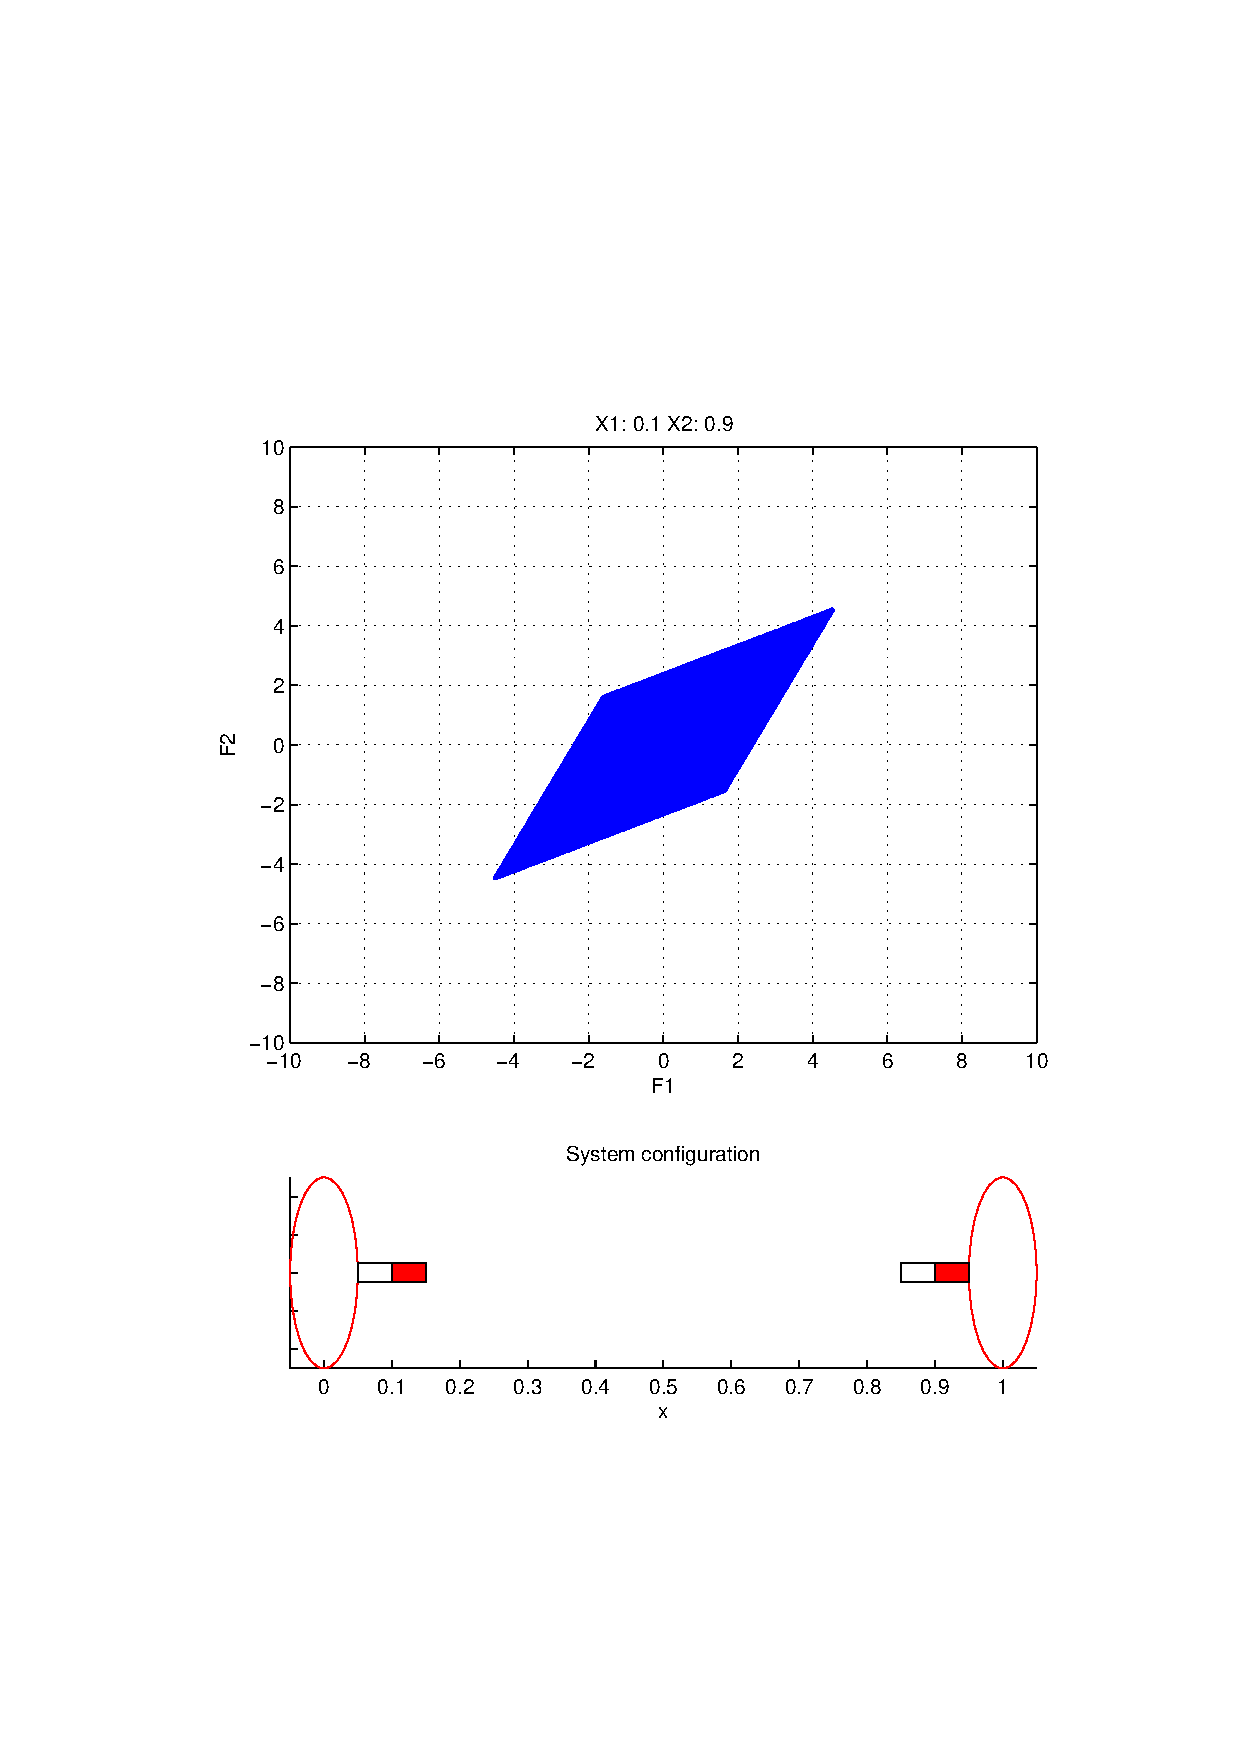
\includegraphics[width=3.5in]{figures/X11X29_Fplot.pdf}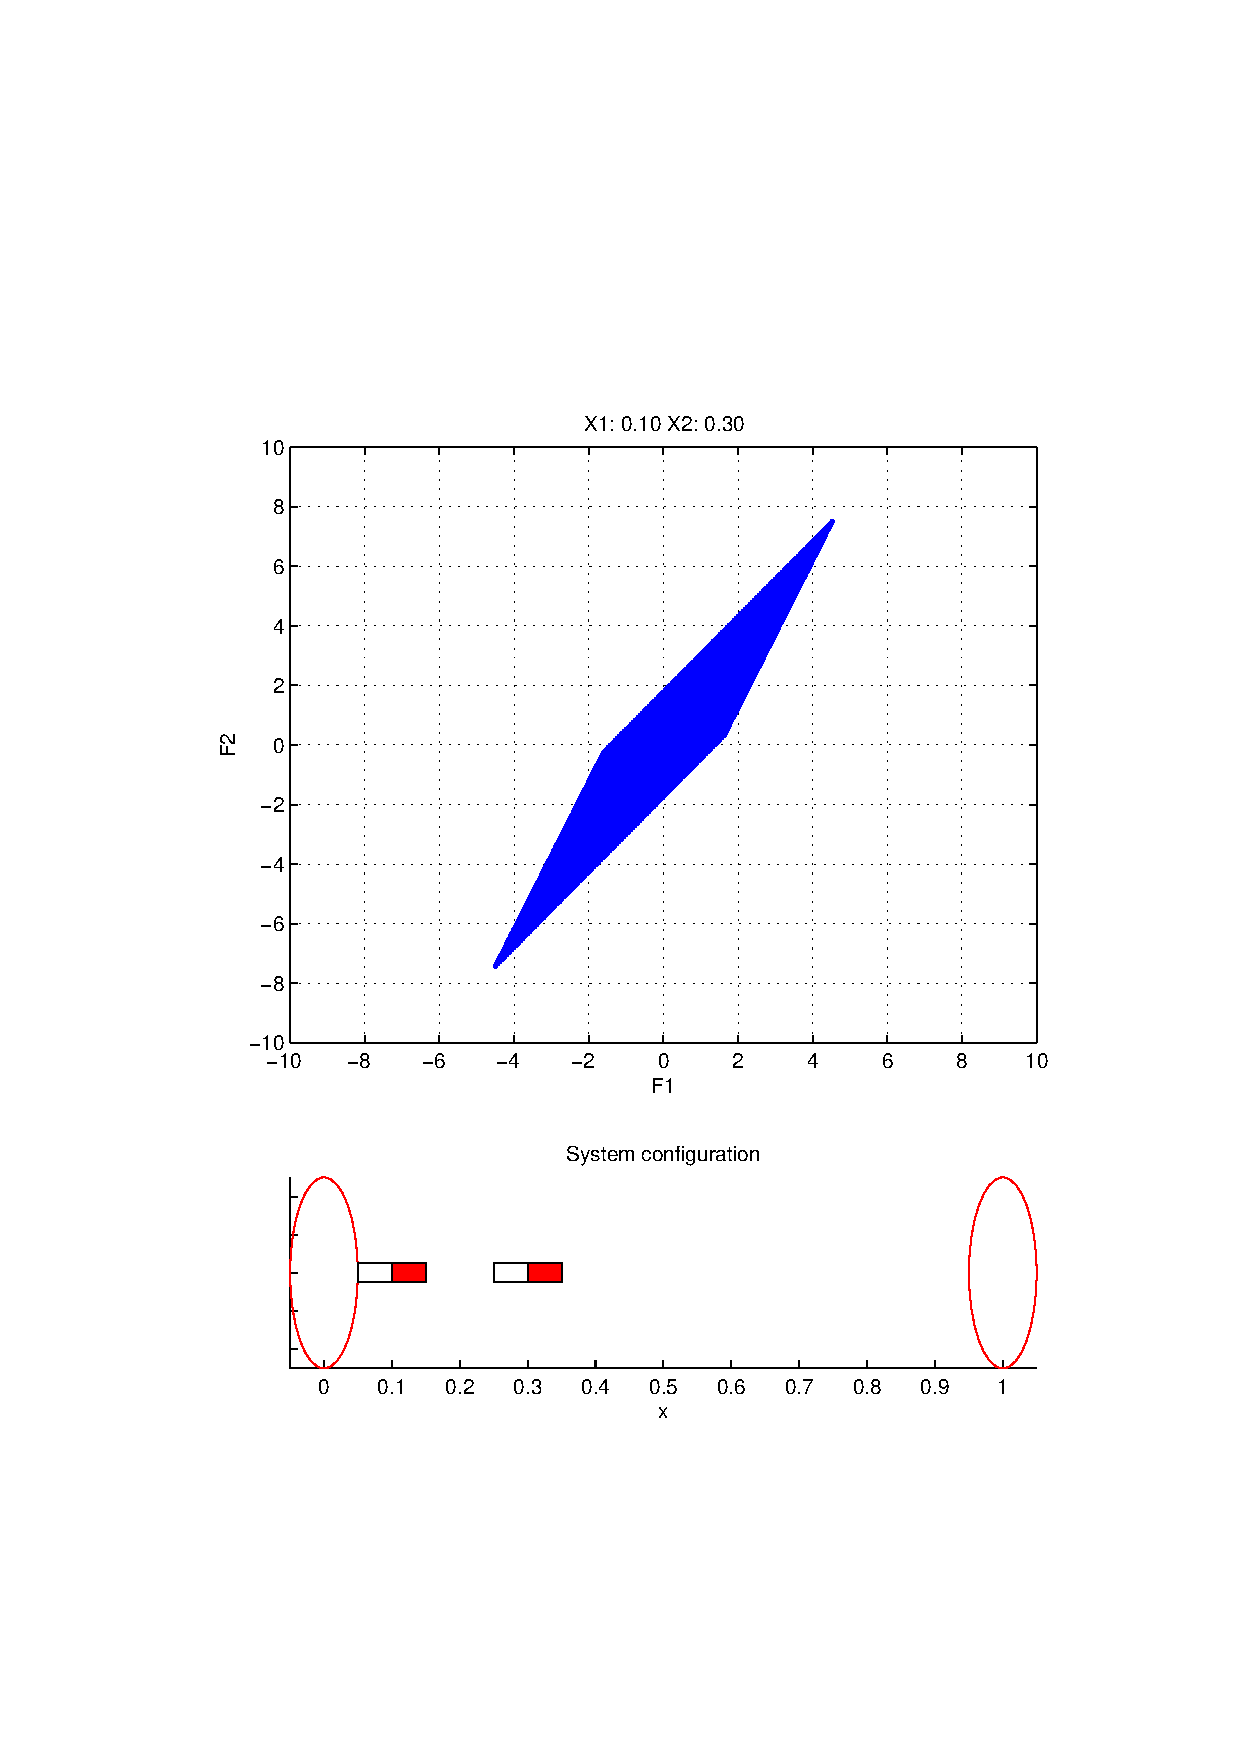
\includegraphics[width=3.5in]{figures/X11X23_Fplot.pdf}

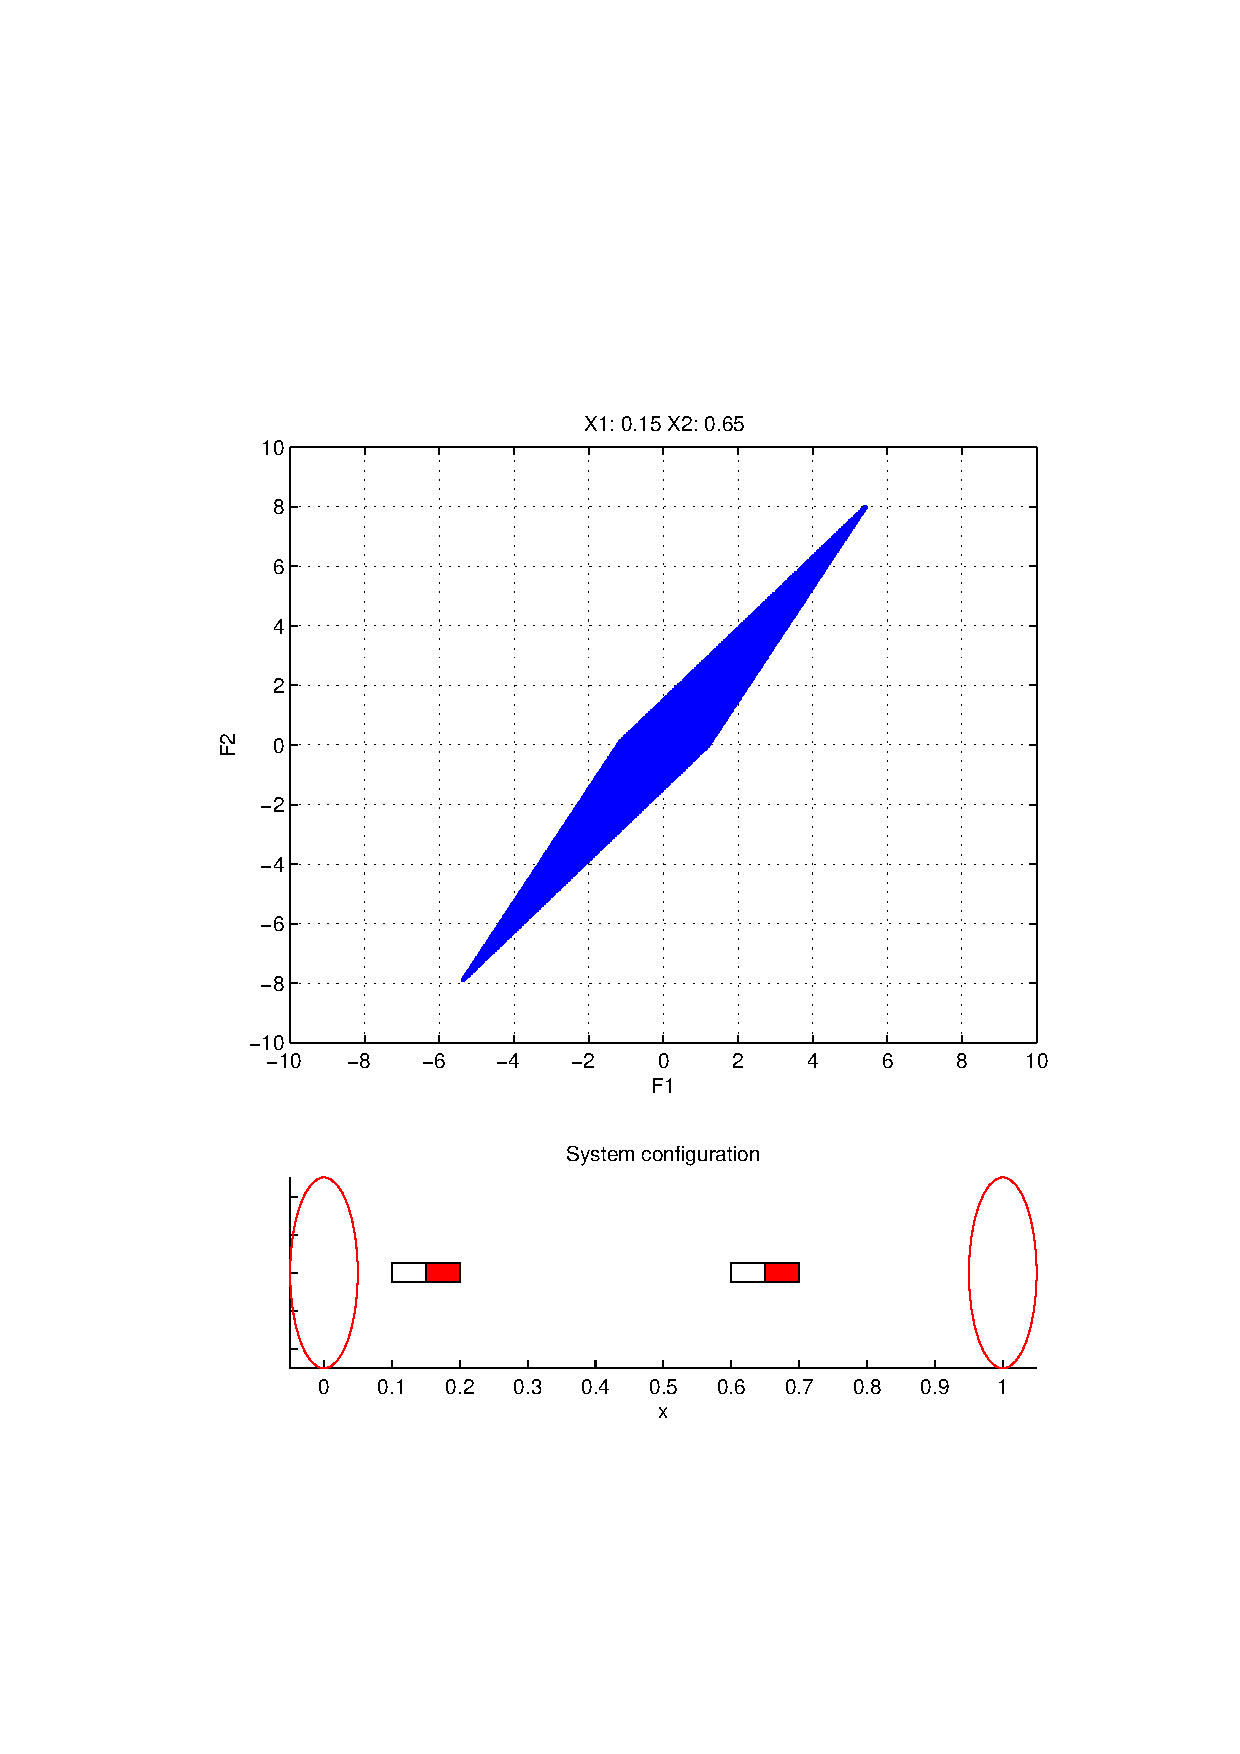
\includegraphics[width=3.5in]{figures/X115X265_Fplot.pdf}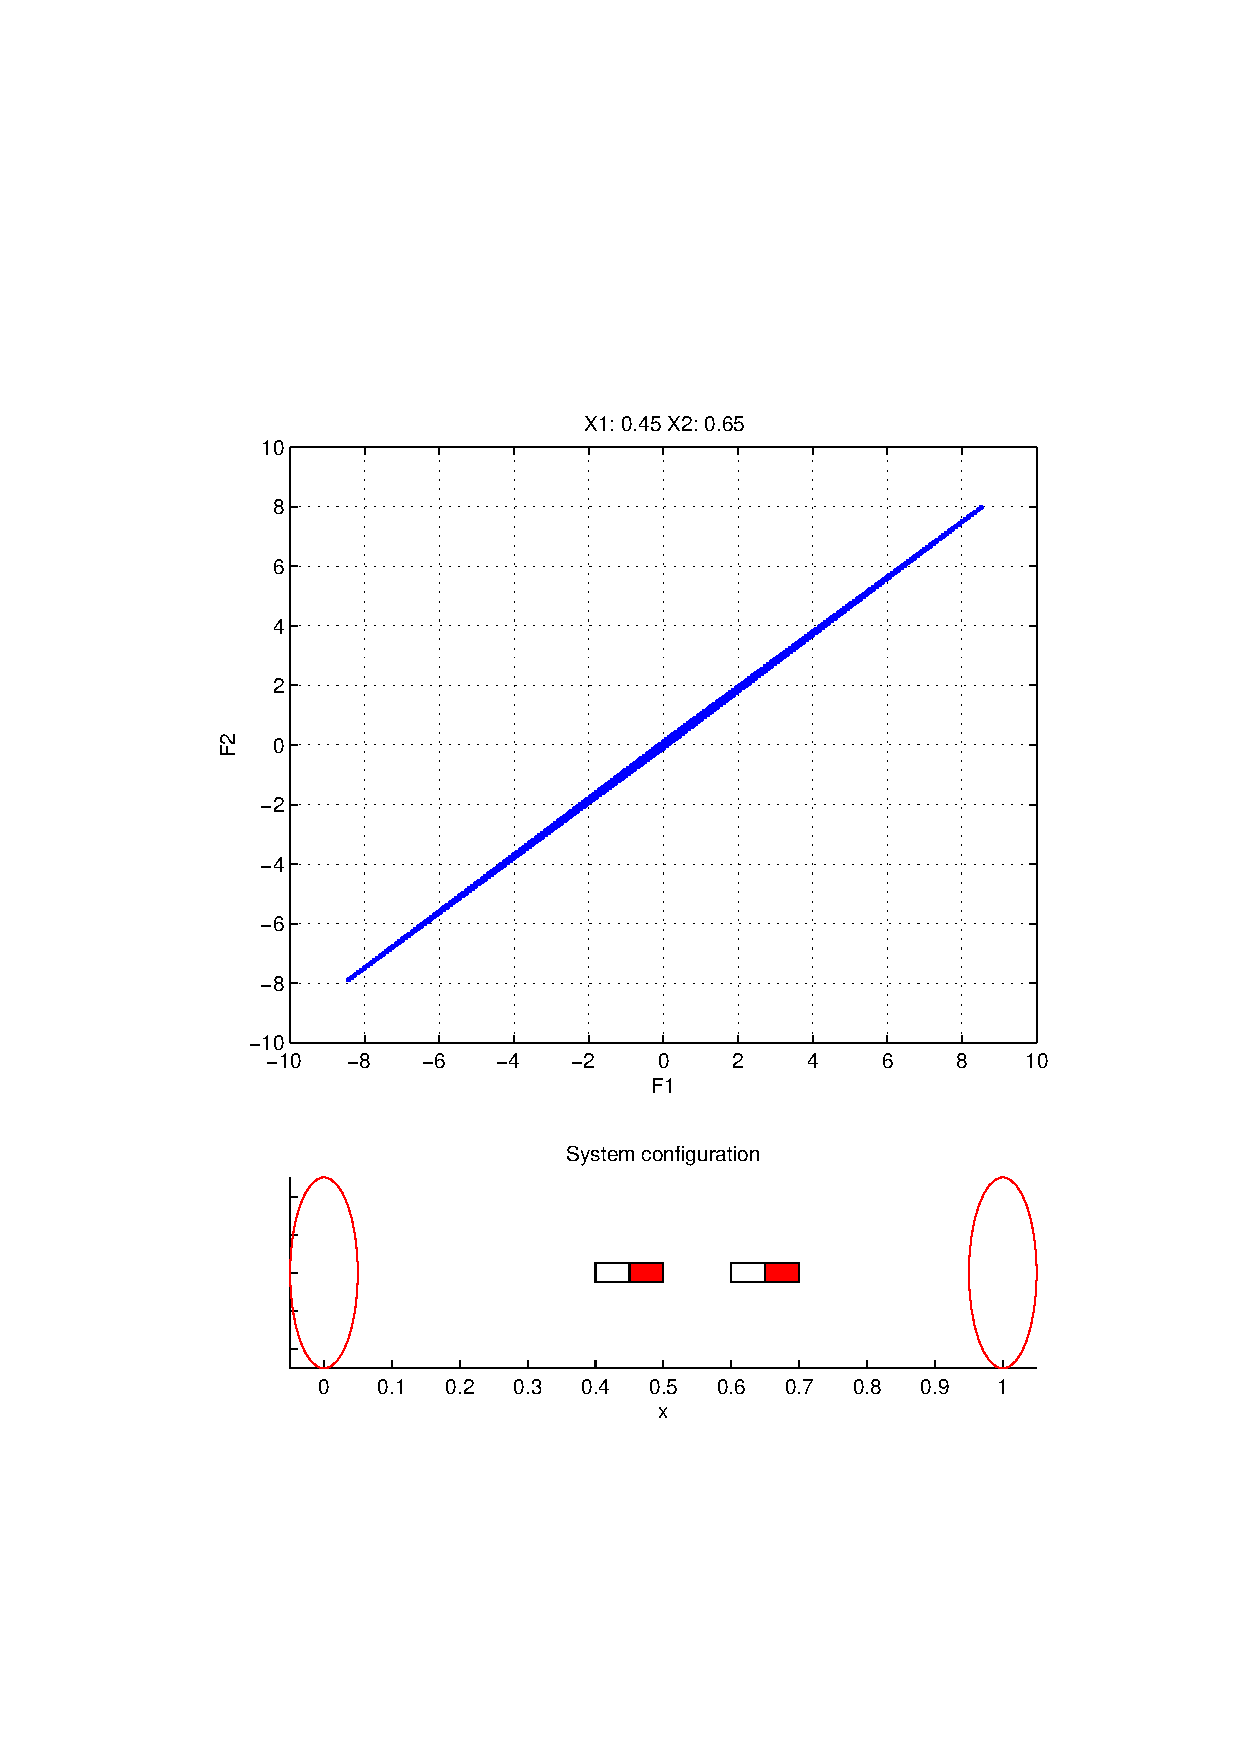
\includegraphics[width=3.5in]{figures/X145X265_Fplot.pdf}
\end{center}

\subsection{2-Opposing Permanent Magnets and 2-Electromagnetic Coil system}
By orienting the magnets in opposing direction such that $\vec{m_1} = -\vec{m_2}$, equation \ref{eq:ForceMatrix_nondim} becomes: 
\begin{equation}
\begin{bmatrix}
	\tilde{F}_{x,1}\\[0.3em]
	\tilde{F}_{x,2}	
\end{bmatrix}
=
\begin{bmatrix}
			-\frac{3\mu}{2} \frac{\tilde{x}_1}{\left(\tilde{x}_1^2 + 1 \right)^{\frac{5}{2}}}  & -\frac{3\mu}{2}\frac{\frac{1}{\alpha}\left(\alpha\tilde{x_1} - 1 \right)}{\left(\frac{1}{\alpha^2}\left(\alpha \tilde{x_1} - 1 \right)^2 + 1 \right)^{\frac{5}{2}}} & -\left(\tilde{x_2}-\tilde{x_1}\right)^{-2}\\
			\frac{3\mu}{2} \frac{\tilde{x}_2}{\left(\tilde{x}_2^2 + 1 \right)^{\frac{5}{2}}}  & \frac{3\mu}{2}\frac{\frac{1}{\alpha}\left(\alpha\tilde{x_2} - 1 \right)}{\left(\frac{1}{\alpha^2}\left(\alpha \tilde{x_2} - 1 \right)^2 + 1 \right)^{\frac{5}{2}}} & 	\left(\tilde{x_2}-\tilde{x_1}\right)^{-2}\\
\end{bmatrix}
\begin{bmatrix}
	\tilde{I}_1\\ \tilde{I}_2 \\ \frac{\mu_0 m^2}{4 \pi R^2}
\end{bmatrix}
\label{eq:ForceMatrix_nondimopp}
\end{equation}
The A matrix is now:
$ A = \begin{bmatrix}-0.1463  &  0.3063 & -25.00\\
    0.3628 &  -0.3875 &  25.00
\end{bmatrix}   $\\
Carrying out a similar analysis for the realizable forces: 
%% MATLAB plots
\vspace{-0.1in}
\begin{center}
\includegraphics[trim = 0 .5in 0 0,width=3.2in]{figures/Opposing_X1010X2030.pdf}\includegraphics[trim = 0 .5in 0 0,width=3.2in]{figures/Opposing_X1010X2090.pdf}\\
\includegraphics[trim=0 0.5in 0 0,width=3.2in]{figures/Opposing_X1015X2065.pdf}\includegraphics[trim=0 0.5in 0 0,width=3.2in]{figures/Opposing_X1045X2065.pdf}
\end{center}

An additional difference with these opposing magnets is that the equilibrium are stable.  The potential function for magnet 1 differs by just the sign of the term for the force from the permanent magnet, the expression becomes:

$$U_1 = \mu_1\left(\frac{\mu_0 I_1 R_{1}^{2}}{2 \left(x_1^2 + R_1^2 \right)^{\frac{3}{2}}} + \frac{\mu_0 I_2 R_{2}^{2}}{2 \left(\left(x_1 - L \right)^2 + R_2^2 \right)^{\frac{3}{2}}} \right) - \frac{\mu_0 m_1 m_2}{4\pi \left(x_2 - x_1\right)}$$

For a coil separation of L = 0.10 m with coils of radius R = 0.01 
To hold 2 magnets at x = 0.03 and 0.05 m
Current needed: I1 = -0.0502 A, I2 =  0.4709 A 
\begin{figure}[H]
	\centering
	\includegraphics[width=5in]{figures/UF_stable.pdf}
\end{figure}

\section{Simulation of 2 Permanent Magnets and 2-Electromagnetic Coil system}



\section{Analysis of 3 magnet system in 1-D}
To study this system further, we can add another magnet such that there are 3 magnets and 3 electromagnets all aligned axially.  A similar non-dimensional analysis is carried out for this system.  The system of equations is given by:
\begin{center}
\includegraphics[width=5in]{figures/3magdrawing.pdf}
\end{center}

\begin{equation}
\begin{bmatrix}
	\tilde{F}_{x,1}\\[0.3em]
	\tilde{F}_{x,2}\\[0.3em]
	\tilde{F}_{x_3}
\end{bmatrix}
=
\begin{bmatrix}
			-\frac{3\mu}{2} \frac{\tilde{x}_1}{\left(\tilde{x}_1^2 + 1 \right)^{\frac{5}{2}}}  & 
-\frac{3\mu}{2}\frac{\frac{1}{\alpha}\left(\alpha\tilde{x_1} - 1 \right)}{\left(\frac{1}{\alpha^2}\left(\alpha \tilde{x_1} - 1 \right)^2 + 1 \right)^{\frac{5}{2}}} & 
-\frac{3\mu}{2}\frac{\frac{1}{\beta}\left(\alpha\tilde{x_1} - 1 \right)}{\left(\frac{1}{\beta^2}\left(\alpha \tilde{x_1} - 1 \right)^2 + 1 \right)^{\frac{5}{2}}} &
\left(\tilde{x_2}-\tilde{x_1}\right)^{-2} 
+ \left(\tilde{x}_3 - \tilde{x}_1\right)^{-2}\\
			
			\frac{3\mu}{2} \frac{\tilde{x}_2}{\left(\tilde{x}_2^2 + 1 \right)^{\frac{5}{2}}}  & 
\frac{3\mu}{2}\frac{\frac{1}{\alpha}\left(\alpha\tilde{x_2} - 1 \right)}{\left(\frac{1}{\alpha^2}\left(\alpha \tilde{x_2} - 1 \right)^2 + 1 \right)^{\frac{5}{2}}} & 
-\frac{3\mu}{2}\frac{\frac{1}{\beta}\left(\alpha\tilde{x_2} - 1 \right)}{\left(\frac{1}{\beta^2}\left(\alpha \tilde{x_2} - 1 \right)^2 + 1 \right)^{\frac{5}{2}}} &
-\left(\tilde{x_1}-\tilde{x_2}\right)^{-2} +\left(\tilde{x_3}+\tilde{x_2}\right)^{-2} \\

		\frac{3\mu}{2} \frac{\tilde{x}_3}{\left(\tilde{x}_3^2 + 1 \right)^{\frac{5}{2}}}  & 
\frac{3\mu}{2}\frac{\frac{1}{\alpha}\left(\alpha\tilde{x_3} - 1 \right)}{\left(\frac{1}{\alpha^2}\left(\alpha \tilde{x_3} - 1 \right)^2 + 1 \right)^{\frac{5}{2}}} & 
-\frac{3\mu}{2}\frac{\frac{1}{\beta}\left(\alpha\tilde{x_3} - 1 \right)}{\left(\frac{1}{\beta^2}\left(\alpha \tilde{x_3} - 1 \right)^2 + 1 \right)^{\frac{5}{2}}} &
-\left(\tilde{x_1}-\tilde{x_3}\right)^{-2} -\left(\tilde{x_2}+\tilde{x_3}\right)^{-2} \\

\end{bmatrix}
\begin{bmatrix}
	\tilde{I}_1\\ \tilde{I}_2 \\ \tilde{I}_3  \\ \frac{\mu_0 m^2}{4 \pi R^2}
\end{bmatrix}
\label{eq:ForceMatrix_3nondim}
\end{equation}
where, $\alpha = \frac{L_2}{R}$ and $\beta = \frac{L_2}{R}$.

%\section{Analysis of n-magnet system in 1-D}

\section{Bill of Materials for experimental setup}


\end{document}

